\documentclass{article}
\usepackage[utf8]{inputenc}
\setlength{\parindent}{0cm}
\addtolength{\hoffset}{-2cm}
\addtolength{\textwidth}{4cm}
\usepackage[frenchb]{babel}
\usepackage[T1]{fontenc}
\usepackage{hyperref}
\usepackage{graphicx}
\usepackage{afterpage}
\usepackage{minted}

\title{DotAI - Projet de semestre}
\author{Thomas Ibanez}
\makeindex


\begin{document}
\maketitle

\newpage
\tableofcontents

\newpage

\section{Introduction}

Le but de ce projet de semestre est de créer un ensemble de logiciels permettant de présenter les données contenues sur \url{opendota.com} pour le développement d'un logiciel d'apprentissage automatique sur le jeu DotA 2.

\subsection{DotA 2}

DotA 2 est jeu-vidéo multijoueur de type bataille en arène (MOBA) où 2 équipes s'affrontent. Chaque équipe est composée de 5 joueurs chacun controllant un héro choisi parmis les héros disponnibles dans le jeu (il ne s'agit donc pas d'un avatar personnalisable comme dans le cas des MMORPG). A l'heure actuelle le jeu propose 115 héros, chacuns disposant de 5 attaques différentes. La partie se déroule sur une carte symétrique constituté de 3 "lanes" sur lesquelles sont disposées des tours dont voici une vue aérienne: \\
\begin{center}
	\includegraphics[scale=1]{"minimap.png"} 
\end{center}

Chaque équipe commence dans un coin de la carte (en bas à gauche et en haut à droite), le but pour chaque héros est de controler une partie de la carte et détruire les tours ennemies (T) afin d'arriver jusqu'a la base adverse (A) et de la détruire.\\

En plus des héros chaque base va périodiquement créer des "creeps", sortes de petit monstres qui vont se déplacer sur une lane.

\section{Recupération des informations d'OpenDota}

Opendota collecte une quantitée énorme de parties de DotA 2 jouées par des joueurs du monde entier. Le site présente une API permettant la récupération de matchs selon certains critères. Une documentation sur le genre de requêtes faisable est disponible sur \url{https://docs.opendota.com/}. Dans le cadre de se projet, nous allons utiliser un filtre permettant de séléctionner un héros dont on voudrait qu'il soit présent dans le match.\\
Dans un premier temps M. Malaspinas et moi-même pensions que les données étaient directement exploitable depuis opendota, malheureusement c'est plus compliqué. En effet OpenDota stocke uniquement des données statistiques sur la partie jouée mais pas les actions et positions des entités à chaque instant. Heureusement le résultat contient un lien vers un fichier \textit{.dem} qui lui contient toutes ces informations.

\section{Analyse des fichiers .dem}

Les fichiers .dem sont des fichiers contenant toutes les informations dont on pourrait vouloir sur une partie allant de entités présentes sur la carte jusqu'au commentaires audio si disponnibles. Un fichier .dem pour une partie standard ({\raise.17ex\hbox{$\scriptstyle\mathtt{\sim}$}}30 Minutes) pèse {\raise.17ex\hbox{$\scriptstyle\mathtt{\sim}$}}50Mo.

\subsection{Format}

Le format global de ces fichiers est assez simple. DotA utilise protobuf, une technologie de sérialization développée par google, pour encoder ces fichiers. Le protocole est maintenu à jour par l'équipe SteamRE sur \url{https://github.com/SteamRE/SteamKit/tree/master/Resources/Protobufs/dota} \\
Chaque fichier commence par une en-tête, soit "PBDEMS2" pour les replay datant d'après la mise à jour de DotA sur le moteur de jeu Source 2. Soit "PBUFDEM" pour les replay plus anciens. Dans le cadre de ce projet nous nous concentrons uniquement sur les replay d'après Source 2 car ce sont ceux qui sont émis en ce moment.\\
Une fois ce header lu le fichier contient 8-bytes dont l'utilitée n'est pas connue.\\

\subsubsection{Format global}

La suite du fichier est une série d'entrées de ce type:\\
\begin{center}
	\begin{tabular}{| l | l |}
  	 \hline
  		 Nom & Type \\
  	 \hline
 	  	 ID & VarInt  \\
  		 Tick & VarInt  \\
  		 Taille & VarInt \\
  		 Données & Bytes \\
   	\hline
	\end{tabular}
\end{center}

Note: Les varints sont des entiers encodés sur une longeur variable de bits. Cet encocodage est détaillé sur \url{https://developers.google.com/protocol-buffers/docs/encoding#varints} \\

L'ID va indiquer le type du message parmis la liste définie dans le protocole:
\inputminted[breaklines,breaksymbol=, frame=single,label=Messages, stepnumber=1,tabsize=2]{Protobuf}{messages.proto}

La seule exception est \textit{DEM\_IsCompressed} qui n'est pas un type de message mais qui défini un bit (6ème bit) qui s'il est égal à 1, alors le message doit être décompressé via la librairie snappy avant d'être interpreté.\\

Le Tick va définir le moment dans la partie ou le message arrive. \\

Le champ Taille indique la taille en bytes des données de ce message.\\

Une fois ces informations connues nous pouvons lancer le décodage via protobuf afin d'obtenir le message, du moins c'est le cas pour tout les ID sauf DEM\_SignonPacket, DEM\_Packet, DEM\_FullPacket et DEM\_SaveGame. Pour ces messages-ci il va falloir lire les données intégrées.\\

\subsubsection{Données intégrées}

Les données intégrées sont basiquement un message encodé dans un autre message. Dans notre cas un DEM\_Packet et un DEM\_FullPacket sont définis comme: 
\inputminted[breaklines,breaksymbol=, frame=single,label=Packets, stepnumber=1,tabsize=2]{Protobuf}{dem_packet.proto}
Les DEM\_SignonPacket n'ont pas de définition distincte, leur structure est la même qu'un DEM\_Packet.
Les DEM\_FullPacket sont en fait composés d'une \textit{StringTable} et d'un DEM\_Packet qu'il faudra interprêter comme les autres DEM\_Packet.\\

Comme on peut le constater un packet n'est en vérité que composé de numéros de séquences (qui ne sont pas intéressants dans notre cas) et d'une suite de bytes qu'il nous faut interprêter. L'intérprétation de ce champ est la suivante: Il s'agit d'une série de sous-messages dont encodés d'une manière ressemblant au format global du fichier:

\begin{center}
	\begin{tabular}{| l | l |}
  	 \hline
  		 Nom & Type \\
  	 \hline
 	  	 ID & Bitvar  \\
  		 Taille & VarInt \\
  		 Données & Bytes \\
   	\hline
	\end{tabular}
\end{center}

Ce qu'il faut remarqué c'est que l'ID est encodé en tant que "bitvar" et non pas en tant que VarInt. Ce format est un petit peu particulier et implique un désalignement:

\begin{verbatim}
Byte No: |       0       ||       1       ||       2       ||       3       ||      4  //
Bit No:  |0 1 2 3|4 5 6 7||0 1 2 3|4 5 6 7||0 1 2 3|4 5 6 7||0 1 2 3|4 5 6 7||0 1      // 
         |-------|-------||-------|-------||-------|-------||-------|-------||---     //
Valeur:  |X Y 0 0|0 0 1 1||1 1 2 2|2 2 3 3||3 3 3 3|3 3 3 3||3 3 3 3|3 3 3 3||3 3     //
\end{verbatim}

Les bits "X", "Y" et "0" doivent obligatoirement être lus. Ensuite: 
\begin{itemize}
\item Si Y vaut 1, il faut lire 4 bits supplémentaires (les bits "1")
\item Si X vaut 1, il faut lire 8 bits supplémentaires (les bits "1" et "2")
\item Si X et Y valent 1, il faut lire 28 bits supplémentaires (les bits "1", "2" et "3")
\end{itemize}
\vspace*{\baselineskip}
Note: Comme on peut le constater, la lecture de cette variable ne s'arrête non pas à la fin d'un byte mais bel et bien au millieu. Nous ne sommes donc plus alignés sur une base de 8 bits ce qui m'a obligé à créer un flux de lecture bit par bit au lieu d'utiliser un des flux disponnibles avec java qui sont tous byte par byte.
\vspace*{\baselineskip}\\
La valeur est ensuite construite de la manière suivante: Les 4 bits "0" sont les bits de poids faible, les autres bits restent dans l'ordre dans lequel ils sont écrits (les "1" en poids fort).\\

Le champs taille défini la taille des données de ce sous-packet. Les données sont à nouveau une structure encodée via protobuf, cette structure peut être de type NET\_Message ou SVC\_Message (également d'autres types possible mais ils ne nous intéressent pas). \\

Voici les enums SVC\_Messages et NET\_Messages:

\inputminted[breaklines,breaksymbol=, frame=single,label=Messages, stepnumber=1,tabsize=2]{Protobuf}{netmessages.proto}

Dans ce projet, étant donné que nous ne cherchons pas à créer un interpreteur complet, ce sont les messages svc\_CreateStringTable, svc\_UpdateStringTable, svc\_PacketEntities et svc\_ServerInfo qui vont nous intéresser par le suite. 

\subsection{Données}

Revenons au début du fichier, directement après le magic et les 8-bytes à sauter nous allons trouver un message de type DEM\_FileHeader. Ce message contient des méta-données sur le fichier, par exemple:
\begin{verbatim}
demo_file_stamp: "PBDEMS2\000"
network_protocol: 44
server_name: "Valve Dota 2 Europe Server (srcds122.133.57)"
client_name: "SourceTV Demo"
map_name: "start"
game_directory: "/opt/srcds/dota/dota_v2432/dota"
fullpackets_version: 2
allow_clientside_entities: true
allow_clientside_particles: true
addons: ""
\end{verbatim}
Ces informations ne nous sont cependant pas utiles.\\
Nous trouvons ensuite une série de DEM\_SignonPacket, l'un d'entre eux contient un sous-message de type svc\_ServerInfo dont voici la structure:
\inputminted[breaklines,breaksymbol=, frame=single,label=ServerInfo, stepnumber=1,tabsize=2]{Protobuf}{serverinfo.proto}
Le champ game\_dir va nous permettre de déterminer la version de DotA 2 utilisée, ce qui nous sera utile par la suite. Le contenu du champ ressemble à ça "/opt/srcds/dota/dota\_v2432/dota" (à noter que ce champ est également présent dans le message DEM\_FileHeader. La partie qui nous interesse est "v2432" qui nous indique que le replay à été créer avec la version 2432 de DotA 2.\\

Nous trouvons ensuite des DEM\_Packets qui contiennent des sous-messages de type svc\_CreateStringTable qui vont servir, comme leur nom l'indique à créer des "String Tables".

\subsubsection{String Tables}

Une String Table est une table nomée, composée d'une série d'entrées ayant un index (entier), une clef (chaine de caractères) et une valeur (chaine de bytes) bien que le clef comme la valeur puisse ne pas être définie (null). Voici pour illustrer une petite partie de la String Table "EntityNames" (la table entière contient 251 entrées)
\begin{center}
	\begin{tabular}{| l | l | l |}
  	 \hline
  		 Index & Clef & Valeur\\
  	 \hline
 	  	 24 & dark\_troll\_warlord\_ensnare & null  \\
  		 25 & dark\_troll\_warlord\_raise\_dead & null \\
  		 26 & polar\_furbolg\_ursa\_warrior\_thunder\_clap & null \\
   	\hline
	\end{tabular}
\end{center}

Cependant, pour ce projet la seule table qui va nous intéresser est la table "instancebaseline" qui contient les identifiants de toutes les entités qui ont des propriétés à lire avant leur création.\\

La totalité du contenu de la String Table est englobé dans le champ $StringData$, cependant il est possible que ce champ soit compressé avec la librairie Snappy pour les replay plus récents ou avec LZSS pour les plus anciens. Pour savoir quelle méthode est utilisée on peut vérifier si les 4 premiers bytes composent la chaine de caractères "LZSS".\\
Une fois décompressé si besoin nous pouvons commencer la lecture, il nous faut dans un premier temps déclarer un buffer circulaire de 32 éléments qui va constituer un historique des clefs lues.\\

\afterpage{%
\begin{figure}[!htbp]
\centering
\vspace*{-3cm}
\thispagestyle{empty}
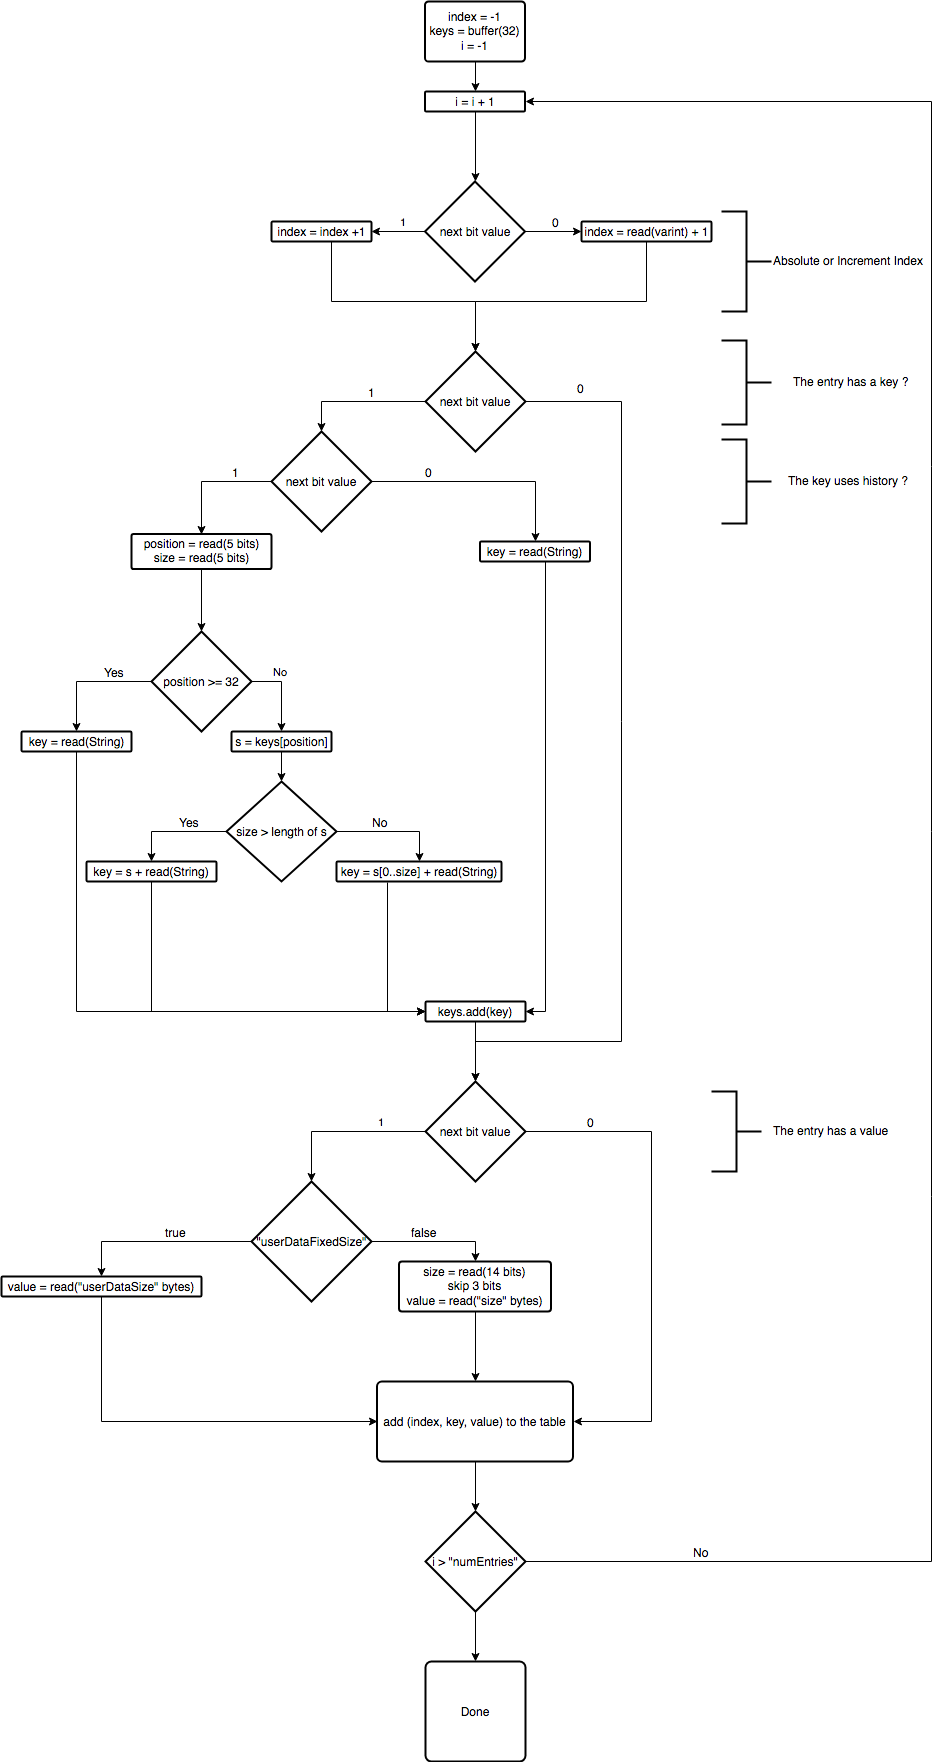
\includegraphics[scale=0.42]{st.png}
\end{figure}
\clearpage
}
\newpage

Une fois toutes ces String tables lues nous allons recevoir un packet contenant les "Send Tables" qu'il va falloir lire également.

\subsubsection{Send Tables}

La définition d'une SendTable est très simple:
\inputminted[breaklines,breaksymbol=, frame=single,label=SendTable, stepnumber=1,tabsize=2]{Protobuf}{sendtable.proto}
Comme on peut le constater il n'y a qu'un champ $data$ qui est une suite de bytes, il va donc falloir le décoder.\\
Heureusement le décodage du champ $data$ est simple, il faut d'abort lire un varint qui va nous indiquez une taille, puis lire cette taille (en bytes) afin d'obtenir une structure de type svc\_FlattenedSerializer

\inputminted[breaklines,breaksymbol=, frame=single,label=FlattenedSerializer, stepnumber=1,tabsize=2]{Protobuf}{flattened.proto}

Les flattened serializers vont nous permettre de connaitre toutes les structures qui vont être lues par la suite, les champs qui les composent et leurs types respectifs. En revanche ils n'expliquent en rien la façon dont il faudra lire les différents types.\\
Voici un exemple de structure (CBodyComponentBaseModelEntity) et ses champs avec leurs types.
\begin{verbatim}
Serializer: CBodyComponentBaseModelEntity
    m_cellX uint16
    m_cellY uint16
    m_cellZ uint16
    m_vecX CNetworkedQuantizedFloat
    m_vecY CNetworkedQuantizedFloat
    m_vecZ CNetworkedQuantizedFloat
    m_hParent CGameSceneNodeHandle
    m_angRotation QAngle
    m_flScale float32
    m_nOutsideWorld uint16
    m_hModel CStrongHandle< InfoForResourceTypeCModel >
    m_MeshGroupMask uint64
    m_nDebugIndex int32
    m_nIdealMotionType int8
    m_ProceduralTargetContexts CUtlVector< CNetworkedIKProceduralTargetContext >
    m_name CUtlStringToken
    m_hierarchyAttachName CUtlStringToken
    m_bIsRenderingEnabled bool
    m_bIsAnimationEnabled bool
    m_materialGroup CUtlStringToken
    m_nHitboxSet uint8
\end{verbatim}

A noter que certains types ne sont pas atomiques mais référencent une autre structure.\\
La manière de décoder chaque type est définie dans la classe $Decoders$ du programme. Il y actuellement 15 décodeurs implémentés.\\

\subsubsection{ClassInfos}

Les classinfos sont une information essentielle au décodage du fichier, en effet chaque fois qu'une entité est réferencée, au lieu de l'obtenir par son nom qui peut être très long comme "CDOTA\_Ability\_Alchemist\_UnstableConcoctionThrow" (48 bytes - 384 bits) le fichier va se servir d'un indentifiant de type nombre entier contenu entre 0 et 754 pour les fichiers récents donc seulement 10 bits (donc un gain de 374 bits à chaque référence de "CDOTA\_Ability\_Alchemist\_UnstableConcoctionThrow").\\

Voici le format de ce message:
\inputminted[breaklines,breaksymbol=, frame=single,label=ClassInfos, stepnumber=1,tabsize=2]{Protobuf}{classinfo.proto}

Il s'agit donc d'une série d'entrées contenant un indentifiant, un nom réseau et nom de table. L'identifiant est le nombre qui permettra de réferencer l'entité par la suite. Le nom réseau est le nom complet de l'entité qui permet également de la retrouver dans les StringTables. Le nom de table ne sert à rien, il n'est d'ailleurs jamais défini pour aucune des entrées, il est possible que ce soit un reste d'une ancienne version du protocole où les deux noms étaient distinct.\\

Une fois les classinfos lues. Nous allons pouvoir passez au décodage des entités, cependant avant de pouvoir le faire il va falloir définir les propriétés des entités essentielles (celles qui étaient dans le String Table "instancebaseline"). \\
Pour ce faire nous allons parcourir les valeur (champ $value$) de chacune des entrées de cette table et les décoder comme propriétés de cette entité, bien que l'entité à proprement parler n'existe pas encore.

\subsubsection{Propriétés}

La lecture des propriétés est essentielle, mais c'est également la plus compliquée. En effet afin de lire les propriétés d'une entité, il faut 3 choses, une flux de bits (non-aligné), un serialiseur (trouvé depuis les send tables) et un arbre d'Huffman. 

\subsubsection{PacketEntities}

Les données intégrées de type svc\_PacketEntities forment le coeur du fichier. En effet dans ce format tout est une entité, du "monde" dans lequel le jeu se passe, aux héros controlés par les joueurs en passant par les équipes.\\
Voici la structure de ce type de message:
\inputminted[breaklines,breaksymbol=, frame=single,label=Entities, stepnumber=1,tabsize=2]{Protobuf}{entities.proto}

Les données sur l'entité sont contenue dans le champ $entity\_data$ qui est de type bytes, il va donc falloir décoder de manière particulière ces données. 

\end{document}
